% book example for classicthesis.sty
\documentclass[11pt,a5paper,footinclude=true,headinclude=true]{scrbook} % KOMA-Script book
\usepackage[T1]{fontenc}                
\usepackage{lipsum}
\usepackage[linedheaders,parts,pdfspacing]{classicthesis} % ,manychapters
%\usepackage[osf]{libertine}
\usepackage{amsthm}
\usepackage{graphicx}
\graphicspath{ {./images/} }
\usepackage{wrapfig}

\usepackage[
backend=biber,
style=numeric,
sorting=ynt
]{biblatex}



\addbibresource{bibliography.bib}

\begin{document}

	
	\tableofcontents 


    
\chapter{Installing tMAVEN}
tMAVEN is a free open-source software available to anyone looking to comparatively analyze single molecule time-series data. The easiest way to Install tMAVEN is to navigate to \url{https://github.com/GonzalezBiophysicsLab/tmaven}, go to releases and install the latest .dmg for Mac or .msi for Windows. 
\\


Otherwise, users can also do a manual installation (not recommended) also oulined at \url{https://gonzalezbiophysicslab.github.io/tmaven/install.html}. There are a few softwares necessary for installation: 
\begin{itemize}
    \item Python, which is available for download at many cites, we recommend miniconda which may be installed at \url{https://docs.conda.io/en/latest/miniconda.html}
    \item A GitHub account which may be made at \url{https://github.com/join} and then they must generate an ssh key and add it to their git hub account as shown at \url{https://www.inmotionhosting.com/support/server/ssh/how-to- add-ssh-keys-to-your-github-account/} an HTTPS key may also be used. 
    
\end{itemize}

If this software is already set up, a user must do the following in sequence: 
\begin{itemize}
    \item navigate to the tMAVEN repository at \url{https://github.com/GonzalezBiophysicsLab/tmaven}, and clone the repository using an ssh key (discussed above) or an HTTPS key.
    \item open terminal navigate to the tMAVEN folder and enter the command "pip install -e ." and select yes/enter to any subsequent requests.
\end{itemize} 
    
\chapter{Navigating tMAVEN}

\section{Loading Data}
    
        tMAVEN can support ASCII, SMD\cite{SMD} (HDF5 based), raw HDF5, and SPARTAN files. Load data by hitting File/\textbf{Load}, select file type, and then the file itself. Note that class, pre/post etc. files may be uploaded separately. The default upload settings are for SMD files, so if using ASCII files, the upload setting must be chosen through the menus File/Load/Text files (ASCII/UTF)/Raw/[user's format]. In this section, N refers to number of traces, T to number of time points and C to number of  colors. Collation axis (0 or 1) refers to how the text separates individual traces 
     
       \begin{figure} [h]
           \centering
           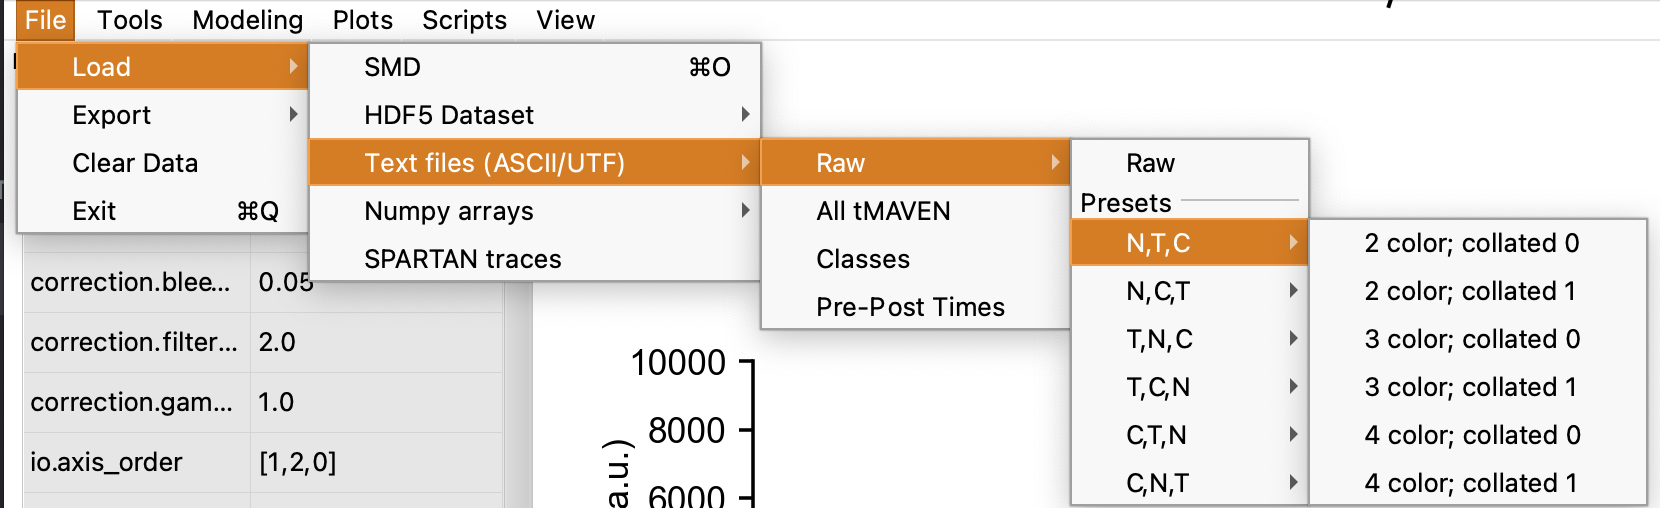
\includegraphics[scale=0.33]{ASCIIupload.png}
           
       \end{figure}
       
    
        %ebfret is n*t and might be csv or tsb delimiter 
     
Note that any preferences using True/False are case sensitive. There is also an \textbf{HDF5 viewer} tool under "View" that the user may find useful.    

\section{The Molecule Table}    
        Navigate to the molecule table View/\textbf{Molecule Table} or hit command T to bring up the molecule table. Notice the columns:
    
     %   \begin{figure} 
     %       \centering
    %        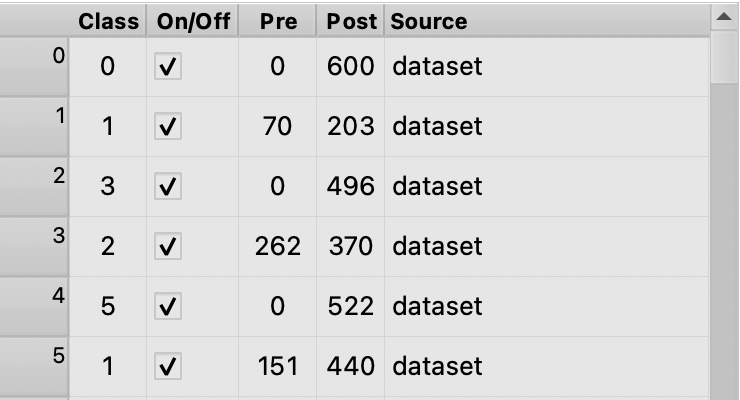
\includegraphics{Molecule Table Sample.png}
    %        \caption{Caption}
    %        \label{fig:my_label}
   %     \end{figure}
   
         \begin{itemize}
         \item Class: the class of the trace, change a trace's class by clicking its row in the molecule table and inputing a number, or simply by clicking around the plot and keying a number.
         \item On/Off: Whether the trace is turned on. By toggling a trace one can easily choose which traces  are included in modeling and plotting features, see section 4. It will also toggle whether the trace is subject to actions like save.
         \item Pre/Post: The range of time each cut trace covers 
         \item Source: If modeling from different datasets, the origin of each trace can be seen here. Note that the class can be assigned separately from the source. 
         \end{itemize}

         
    \begin{figure} [h]
   \centering
   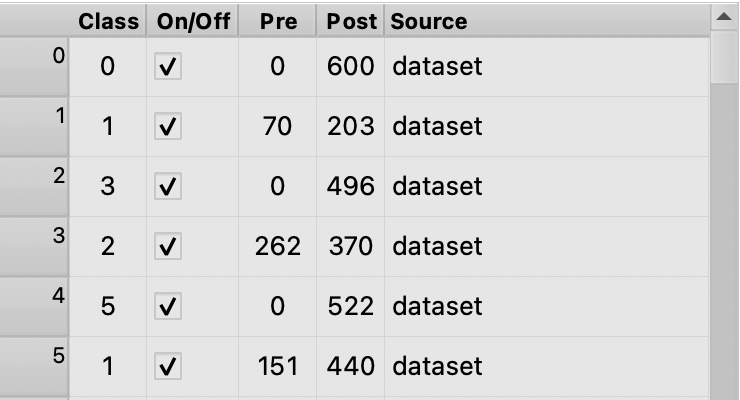
\includegraphics[scale=0.5]{Molecule Table Sample.png}   
   \end{figure}
     Classifying traces is one of the most powerful aspects of tMAVEN. 

  
    \section{Using the UI and Cutting a trace}
    
   
Navigate between traces by scrolling while graph window is selected or by using the scroll underneath the graphs (see figure 1). Notice trace number and class of the graph displayed in the bottom right corner. Aspects of the graph can be adjusted in the graph settings and figure options (see figure 1), or in preferences. Most of these settings are plot.[aspect] and include settings for the axes, subdivision ticks, time scale, and more. The user can always use the View/\textbf{reset GUI} command to set all these settings to default. 
\begin{figure} [h]
    \renewcommand{\figurename}{Figure 1}
    \renewcommand{\thefigure}{}
   \centering
   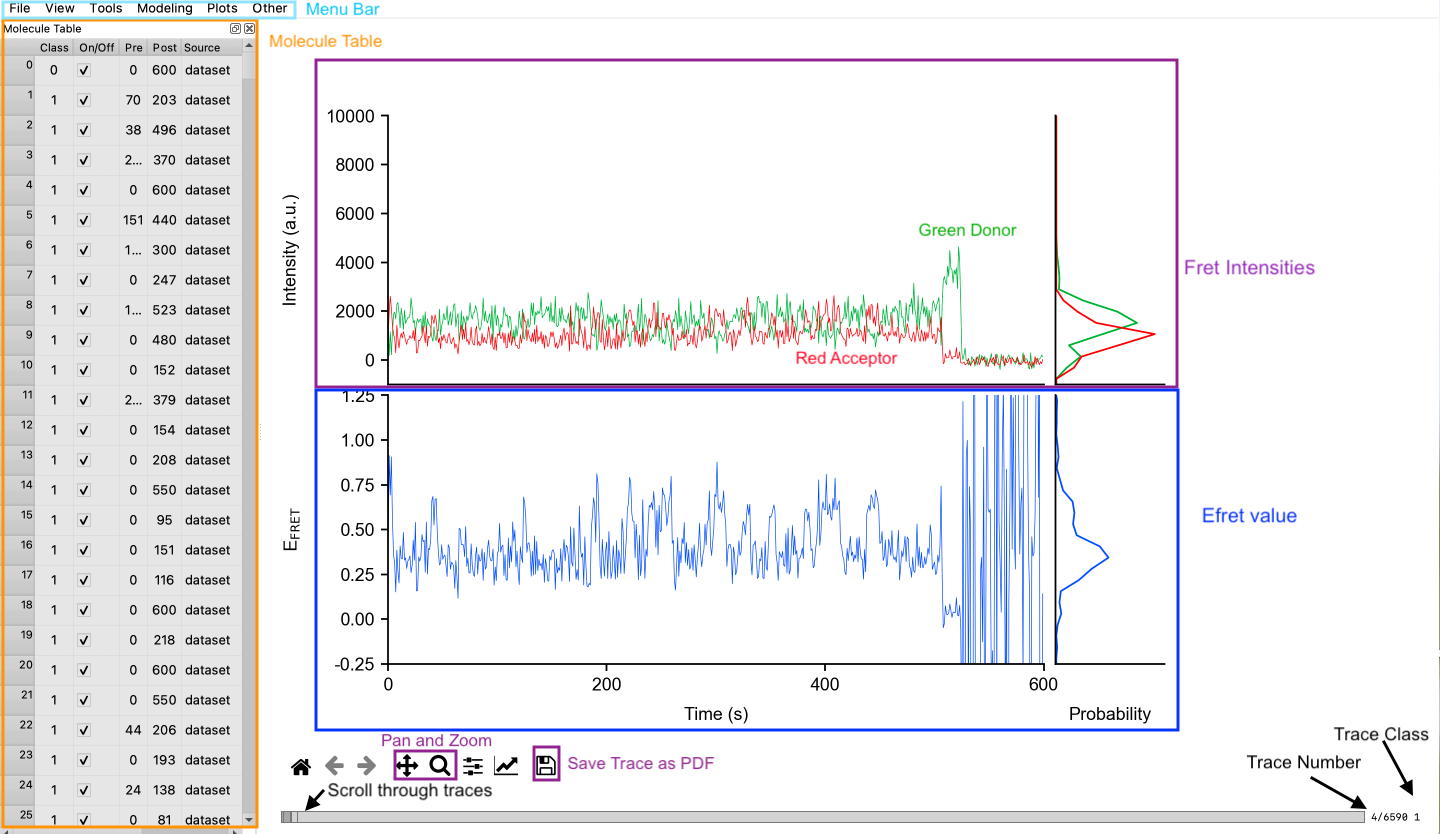
\includegraphics[scale=0.33]{General UI.png}
   \caption{labeled UI after loading a dataset}
   \end{figure}

Most actions in tMAVEN do not alter the raw data of a 
trace, such as gamma and bleed-through corrections. Only cutting traces actually alters the pre and post times which can be seen in the molecule table or on the traces themselves. The user can set the post time by right clicking at the desired point on a graph or left clicking for the pre time. Notice that once a section has been cut out, it appears much fainter on the graph. Reset the pre and post times for a single trace by hitting \textbf{R}. Users can also use the square brackets to increase and decrease the post time by 1 point.

Other tools include the \textbf{pan} and \textbf{zoom} features (see figure 1). Use the zoom tool to select a section of the graph to enlarge and to allow more precise selection of pre/post time. Additionally, hit \textbf{G} to toggle viewing subdivisions on the graph (settings for these can be altered in preferences as described earlier). 
Another useful tool is \textbf{single photobleach detection}, which finds and cuts out photobleaching for only the trace shown. Hit \textbf{P} to apply this tool to the shown trace. Photobleach for all traces is also available and is discussed in section 3.5. 
      %click and right click, use zoom (inspect? tool), graph subdivisions- command g

But before any manual trace picking is done, it is highly recommended that the user employ the preprocessing tools described in section 3.
    
\chapter{Preprocessing}
%    The most basic part of trace picking is determining which traces are serviceable and which blocks of those traces are useful. 
 The tMAVEN tools allow  users to skip a lot of the painful preprocessing by culling bad traces, reordering traces by viability, and adjusting the presentation of those traces without altering the raw data, all of which makes data sets easier to process. These features can be found under "tools", and all should be considered before trace picking to optimize the process. 
\section{Selection}
    Before going through traces users should navigate to tools/ selection/\textbf{order by/cross-correlation} to order traces by cross-correlation since good FRET data corresponds to cross correlated jumps of the donor and acceptor emissions. Notice also the options to \textbf{order b}y and \textbf{Turn on/off} by class.
    One of the greatest strengths of tMAVEN is the ease of classifying and viewing traces with the molecule table (refer to section 1.2). The power to classify traces greatly enhances use of the algorithms discussed in section 4 by the ease with which one  may experiment with inclusion of groups of traces. In this case the user is not forced to go through the whole data set repeatedly. 
    %The reasons to classify traces are (xyz)
\section{Filter Traces}
    The \textbf{Filter Traces} command, found under tools, allows the user to filter traces by signal to background ratio (SBR). An algorithm that identifies photobleaching (see 3.6) is used to determine the parameters of background. Filter Traces then sorts traces by SBR and allows the user to classify or cull those groups. 

    \begin{figure} [h]
    \centering
    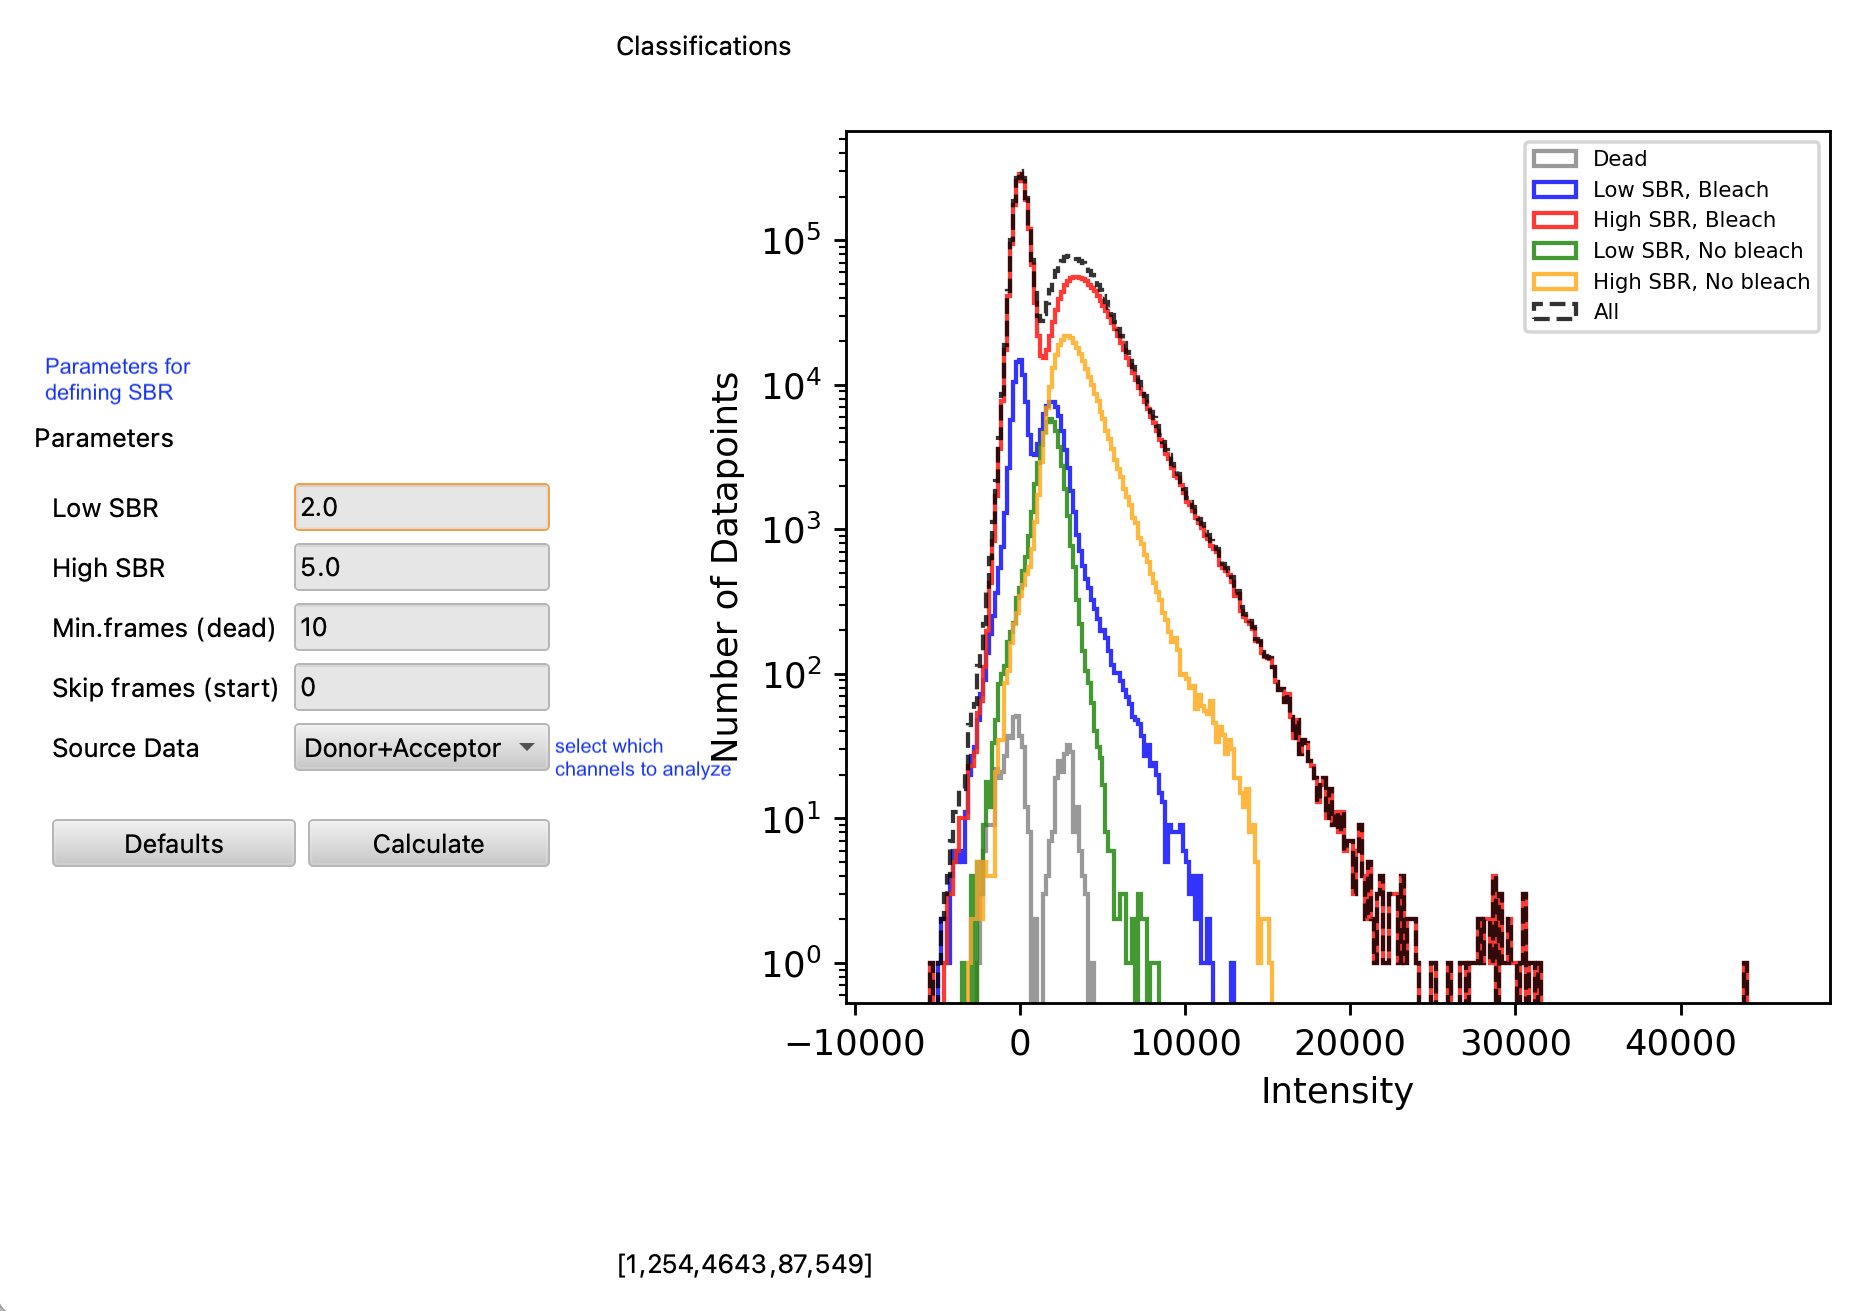
\includegraphics[scale=0.3]{FilterTracesGraphic2.png}
    \caption{A graph like this is generated once calculate is hit. The actual culling/classifying is not completed until the user hits process (see figure 3). The graph enables the user a comprehensive view of their data set}
    \end{figure}
    
    \pagebreak
    Culling in Filter Traces:
    \\
    \begin{wrapfigure}{l}{0.5\textwidth}
    \begin{center}
    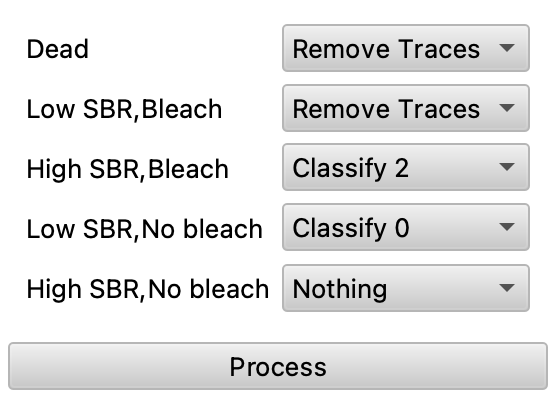
\includegraphics[width=0.45\textwidth]{FilterTracesProcess.png}
    \caption{}
  \end{center}
 
        
    \end{wrapfigure}
    Once calculate is hit and the graph is made, the user can choose what to do with each type of trace (figure 3): ones with low SBR and bleaching, ones with high SBR and bleaching, ones with low SBR and no bleaching, ones with high SBR and no bleaching, and dead traces (traces that bleach before the "minimum frames dead"). Users can repeat the process of filtering and culling until satisfied. 
   
     
   

    
  %  \cleardoublepage\part{Tools}
    
    
    
     
   
    \section{Cull}
    The \textbf{Cull} function under tools is relatively intuitive and allows users to discard traces according to class or a maximum/minimum data point value. The latter functions should be used only after photobleach detection (see section 3.6) lest good traces be culled. The data searched for this function includes only Emissions and not E$_{fret}$ values.
    
    \section{Corrections}
    In this group there are many useful tools such as \textbf{bleedthrough, gamma, and background corrections}. As discussed earlier, the actual data is not altered. The program stores a copy of the given data, and the copy is altered by corrections and displayed. For this reason, the corrections should be applied just once for each time a data set is loaded into tMAVEN.  
   
    \begin{description}
    \item [Bleedthrough corrections] The default bleedthrough correction is set to 5\% and can be adjusted in preferences under correction.bleedthrough.
    \item[Gamma Corrections] The default gamma correction is set to 1 and can be adjusted in preferences under correction.gamma. 
    \item[Background] Background is determined for each trace by the last x frames, alterable in preferences under "correction.backgroundframes," and subtracted from the red emission value.
    
    \end{description}
    \section{Signal Filters}
    Also found under tools/corrections are various signal filters that can make traces much easier to read. All smooth the graphs according to different methods, making the E$_{fret}$ states easier to discern. The filters are found under Tools/Corrections/\textbf{Signal Filters}, and can be removed by resetting corrections under corrections/\textbf{reset}. Reset corrections before switching between signal filters. The width of the filter window's can also be adjusted in preferences by correction.filterwidth which is automatically set to 2. See figure 4 for a look at these filters. 
    \begin{itemize}
        \item \textbf{Gaussian
        \item Wiener 
        \item Median 
        \item 8-pole Bessel} 
        \item \textbf{Chung–Kennedy}\cite{chung} (recommended)  
    \end{itemize}
    
    \begin{figure}
        \centering
        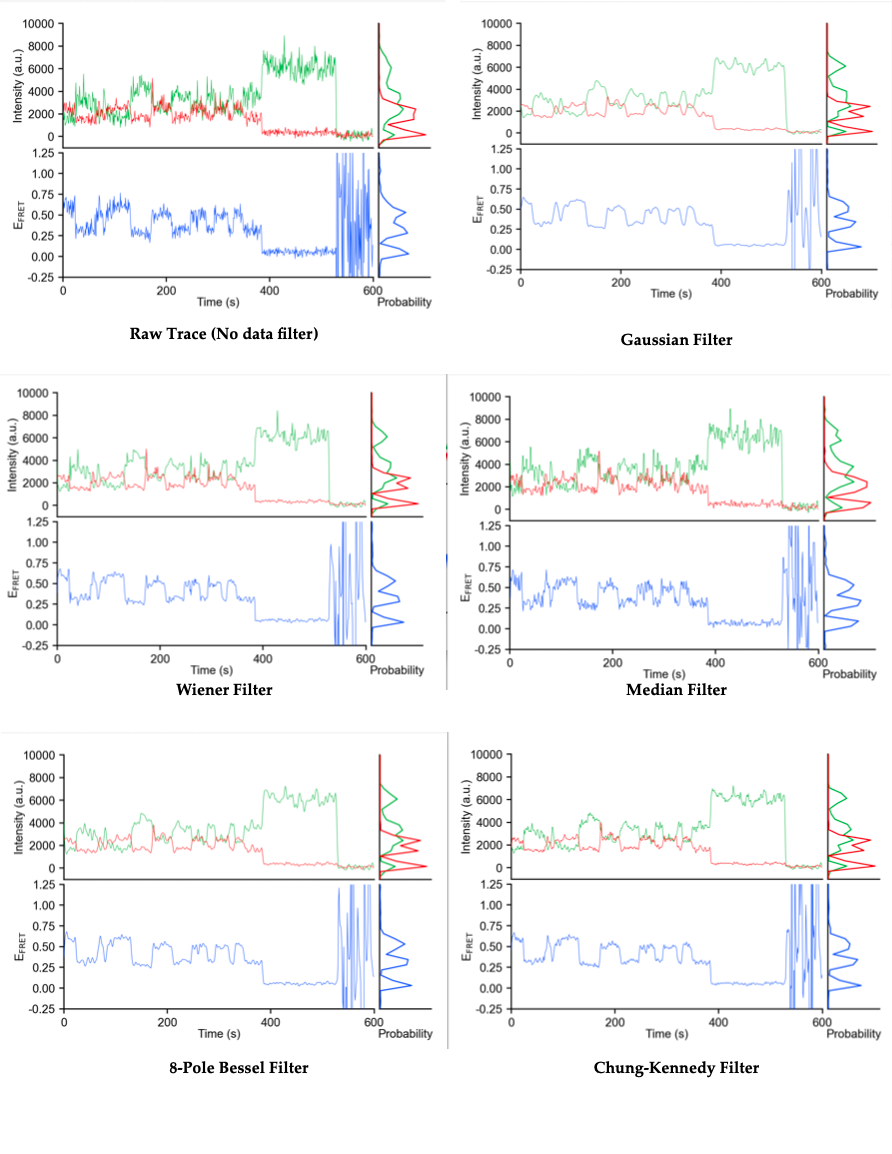
\includegraphics[scale=0.35]{tMAVEN filters Diagram.jpg}
        \caption{The visual effect of the signal filters offered by tMAVEN on the same trace (top left). The benefits of different filters and level of smoothing can be seen here. The Chung-Kennedy filter best maintains the sharp transitions while also reducing noise well. In comparison the Gaussian filter is much more rounded, which makes determining transition times harder.}
        \label{fig:my_label}
    \end{figure}
\section{Photobleaching}
By navigating to tools/photobleach/\textbf{photobleach detection}, the user can run an algorithm that checks each trace for photobleaching and cuts the trace there. Alternatively, users can hit "\textbf{P}" and cut only the trace they are looking at as was discussed in 2.3. The algorithm essentially identifies transitions by maximizing the evidence of a Gaussian between sections of data and placing transitions between those. Photobleaches are then transitions to mean 0 states. 





\chapter{Modeling and Plots}
Possibly the most important feature of tMAVEN is its ability to generate models using various algorithms. Users can also use a variety of plots to assess the performance of those models. For more information on Bayesian inference and use of Hidden Markov Models (HMMs) to model single-molecule data, see \cite{annurev-biophys}. A majority of tMAVEN's algorithms use HMMs which model a time series as transitioning between discrete states hidden by noise. 


\begin{figure}[h]
\centering
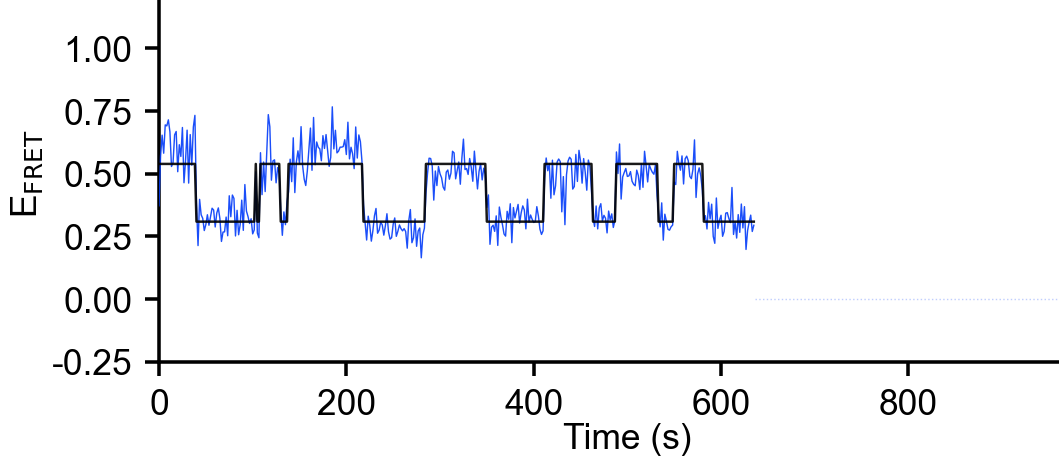
\includegraphics[scale=0.45]{mlHMMex.png}
\caption{After generating a model (see below) tMAVEN shows the idealized trajectory (black line) also called the Viterbi path in black, indicating the most likely state of a molecule at each time point}
\end{figure}


\section{Navigating Between Models} In running any of these algorithms, it may be useful to also check the log, by navigating to View/\textbf{Show Log}. The parameters of a model can be found here, for example: number of determined states, transition matrix, or state means. When generating a model, tMAVEN will only use "on" traces. Viewing the molecule table (1.2) and using the selection tool (2.1) makes toggling molecules on and off much easier. 

Additionally, which model is displayed through idealized trajectories may be selected under Modeling/\textbf{Change Active}. An individual model can be removed with Modeling/\textbf{/Clear Active} or all can be removed with Modeling/\textbf{Remove Models}. Models can be exported or imported as hdf5s with Modeling/\textbf{Export Active} and Modeling/\textbf{Load Active}. If users wish to update the idealized trajectories shown, either after changing pre/post times or including/excluding certain traces, they should click models/\textbf{update idealized}. Note that this will not update the existing model parameters.  

\section{Generating Models}

There are many models to choose from under \textbf{Modeling/FRET Modeling}. One important aspect of these models is whether or not \textbf{Model Selection} is utilized. Without model selection, the user must know and input the number of states, however, if that number is unknown, some algorithms may determine it themselves (see figure 6). These papers elaborate on that selection:
For vbFRET \cite{bronson} and ebFRET \cite{van_de_Meent}
\begin{figure} [h]
    \centering
    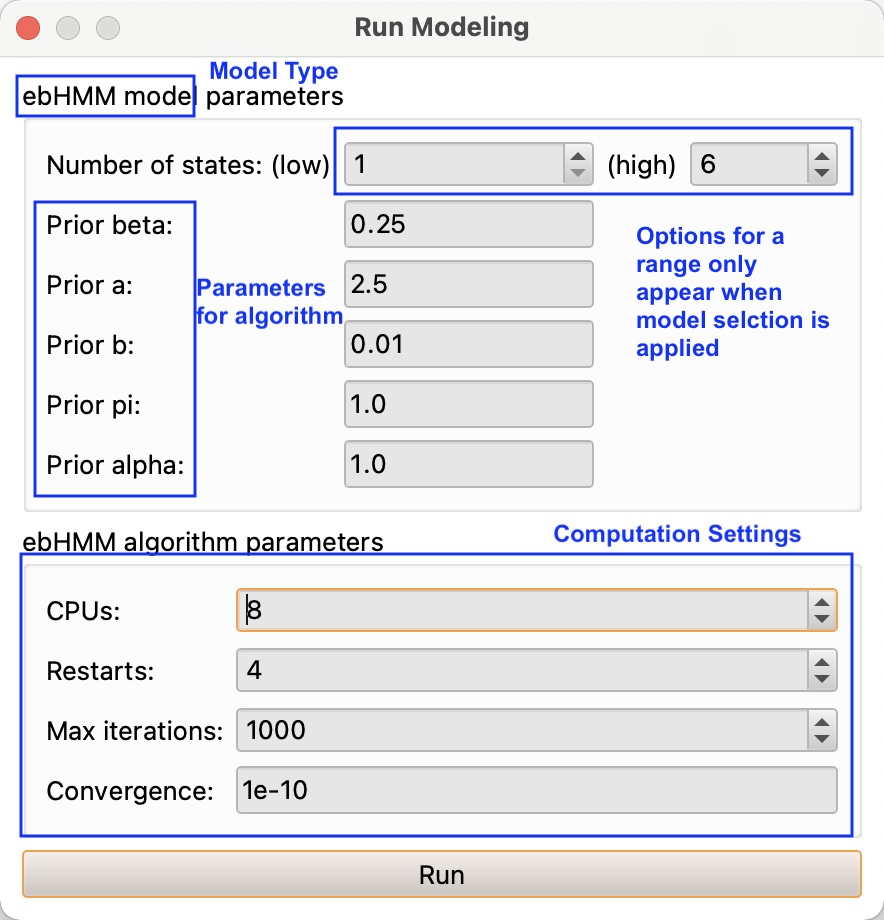
\includegraphics[scale=0.2]{ModelingSettingsEx.jpg}
    \caption{After selecting a model, tMAVEN prompts users to determine some parameters for the modelling algorithms that inform the prior. In most cases these settings need not be changed aside from number of states. The parameters asked for might change depending on the model type. The algorithms in tMAVEN use a Gaussian gamma function with: a as the shape parameter, b as the rate parameter of the gamma distribution parameters, beta as the Gaussian precision parameter, and alpha as the sole parameter of the Dirichlet distribution.\cite{Bishop2006Pattern}}
    \label{fig:my_label}
\end{figure}

When running any model, users also have to input some computational settings (see figure 6). It is recommended to just leave the defaults. The number of restarts corresponds to the number of times the algorithm will restart with different initializations, in order to ensure this state does not affect the final result. The setting for the convergence determines at what relative change in cost function the algorithm will determine convergence has occurred. In case the convergence doesn't occur, the algorithm will cut off after the max iterations.



\section{Generating a Threshold Model}
Under Modeling/FRET Modeling/\textbf{Threshold} is the simplest Model. the threshold model assigns every data point to one of two states dependent on whether it is greater than or less than a user-specified threshold. Threshold models calculate average emission values, means, variances, and fractions of the two states visible in the log.

 \section{Generating a Mixture model}
 
 Under Modeling/FRET/\textbf{Mixtures} are various models that simply cluster the data from all traces either by \textbf{k-means} or by a Gaussian mixture model (GMM) with either a maximum likelihood (\textbf{mlGMM}) or a variational Bayesian (\textbf{vbGMM}) technique \cite{Bishop2006Pattern}.  If the number of states is unknown, users can also choose to use model selection (see section 4.2) with variational Bayesian (\textbf{vbGMM + Model Selection}). Mixture models calculate average emission values, means, variances, and fractions of k states visible in the log.

 \section{Generating a Composite HMM Model}
Composite models under Modeling/FRET Modeling/ \textbf{Composite HMMs} create a hidden Markov model (HMM) for each trace and then cluster them in various ways. This single  clustered model is then used for the idealized paths shown on each trace. 

To generate the HMMs, users can choose either a maximum likelihood algorithm (\textbf{mlHMM})\cite{MCKINNEY20061941} or variational Bayesian algorithm (\textbf{vbHMM}) \cite{bronson}. If the number of states is unknown, users can also choose to use model selection (see 4.2). 

Once HMMs have been generated, they are clustered in various ways: K-means, vbGMM and Threshold which have been elaborated on in sections 4.3 and 4.4. The means, variances and fractions of the states from the clustered model can be found in the log.

\section{Generating Global HMMs}

\textbf{vbConsensus} (variational Bayesian) \cite{TMAVENPAPER} and \textbf{ebHMM} (empiracal Bayesian) \cite{van_de_Meent} are both consensus methods, in that they generate one HMM from the entire data set. In addition to means, variances, and fractions, the consensus methods yield a transition matrix, which may be found in the log or under \textbf{Analyze Dwell Times} as discussed in section 4.7.


\section{Dwell Time Plots and Analysis}
Once a model is run and the number states and their means and transition matrices are calculated, tMAVEN can analyze a data set in terms of dwell times. Before analyzing, go to modeling/\textbf{Analyze Dwell Times}, select your model with "Change Active" and hit calculate (see figure 7). 
To look at a graph for the dwell of a specific state, choose the desired state under rate analysis and input whether it is expected to be a single, double, or triple exponential and hit "\textbf{run}". Under results, the "Rate type" will read "Dwell Analysis", and rates and coefficients will be shown according to the form of the equation selected. For instance a double exponential will show two rates and two coefficients according to the equation $y=A_1e^{-r_1t}+A_2e^{-r_2t}$. 

\begin{figure} 
    \centering
    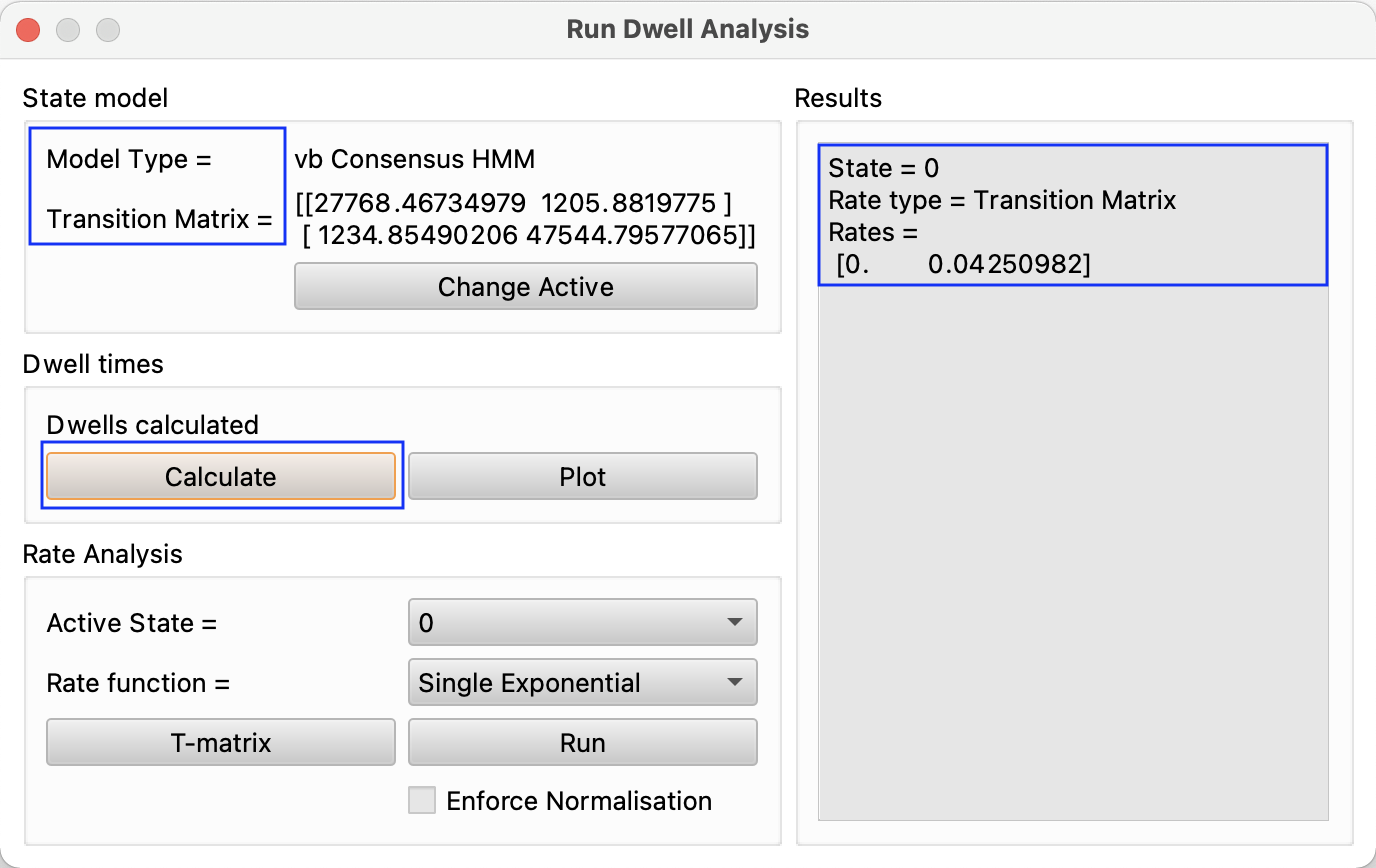
\includegraphics[scale=0.3]{Run Dwell AnalysisFigure.png}
    \caption{Before hitting calculate, make sure the intended model is used by looking at "Model Type" in the top left.} 
    \label{fig:my_label}
\end{figure}
\begin{figure} 
    \centering
    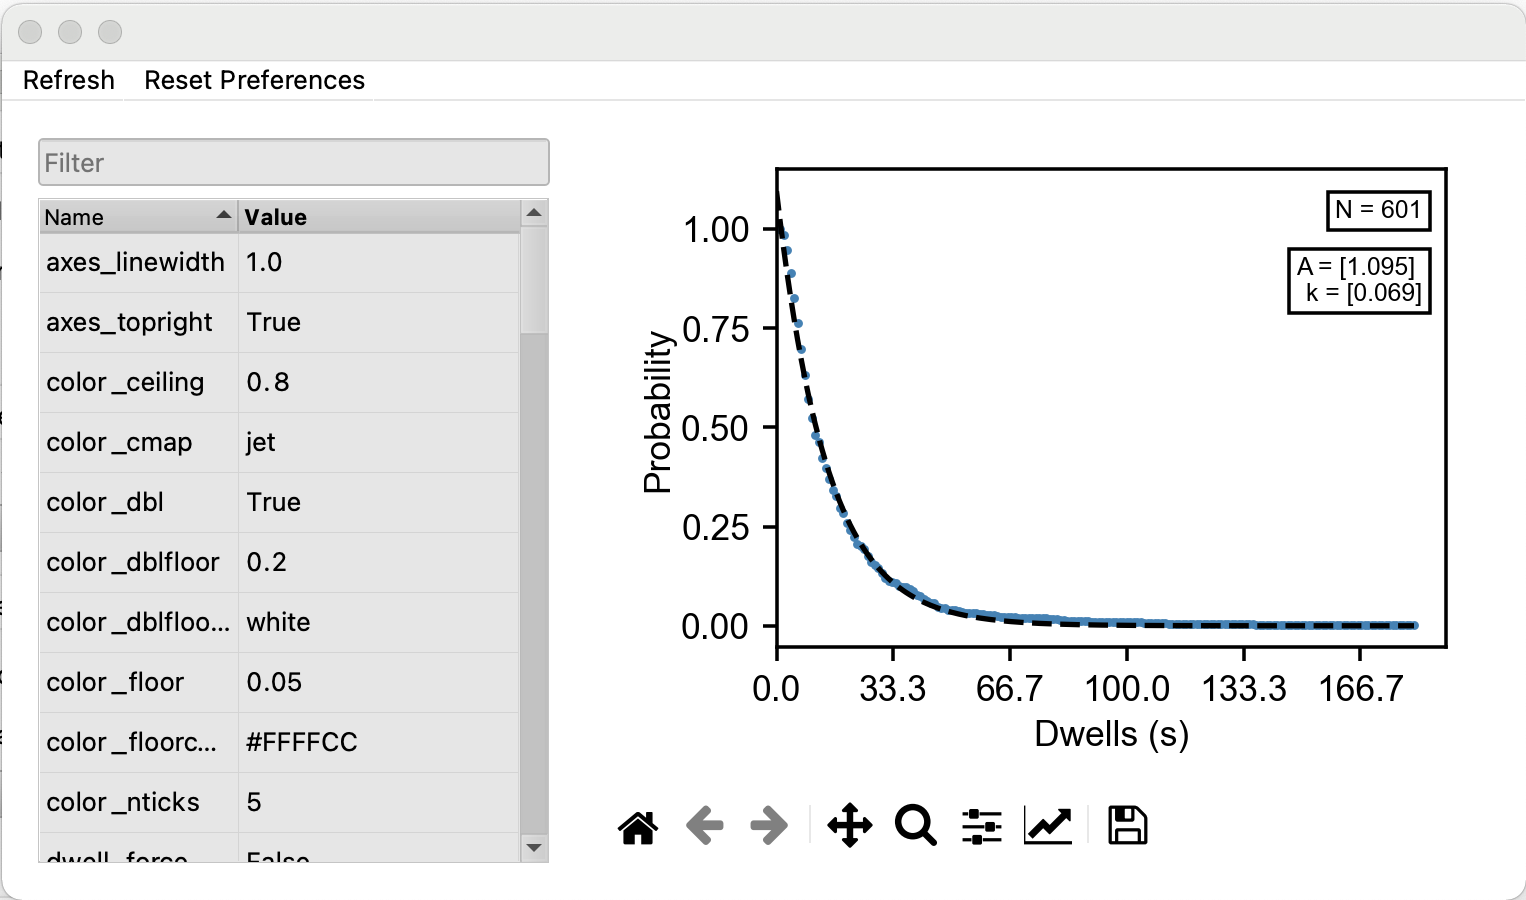
\includegraphics [scale=0.32]{DwellTime Plot.png}
    \caption{A dwell time plot with the data in blue and theoretical dwell graph, from model selected as in figure 7, as a dotted black line. To change the log scale to linear, search on the left for hist$\_$log$\_$y. To toggle the model, search for model$\_$on. To change which state of the model is displayed, search for dwell$\_$state and set to the desired.}
    \label{fig:my_label}
\end{figure}


 
Then, either navigate to plots/\textbf{Dwell Times} or simply hit "\textbf{Plot}" in the Dwell Times section of Run Dwell Analysis (see Figure 7). Now that the plot is made (see figure 8), A histogram of the dwell time is displayed, an exponential decay function. The presets show the y axis on a log scale and the model, theoretical dwell, off. Alter these in the preferences on the left (see figure 8). 

If any series do not appear, or do not update when dwell$\_$state is changed, navigate back to modeling/analyze dwell times and hit calculate again, turn off and on the active model, or hit refresh in the top left corner of the dwell time plot (figure 8).


\section{One-Dimensional Histograms}
The histogram feature of tMAVEN is primarily useful for visualization of data and not diagnostics. Navigate to Plots/\textbf{FRET hist 1D} to generate a one-dimensional histogram of all E$_{fret}$ emission data, the peaks represent states and should look like k gaussians. 

 \begin{figure} [h]
     \centering
     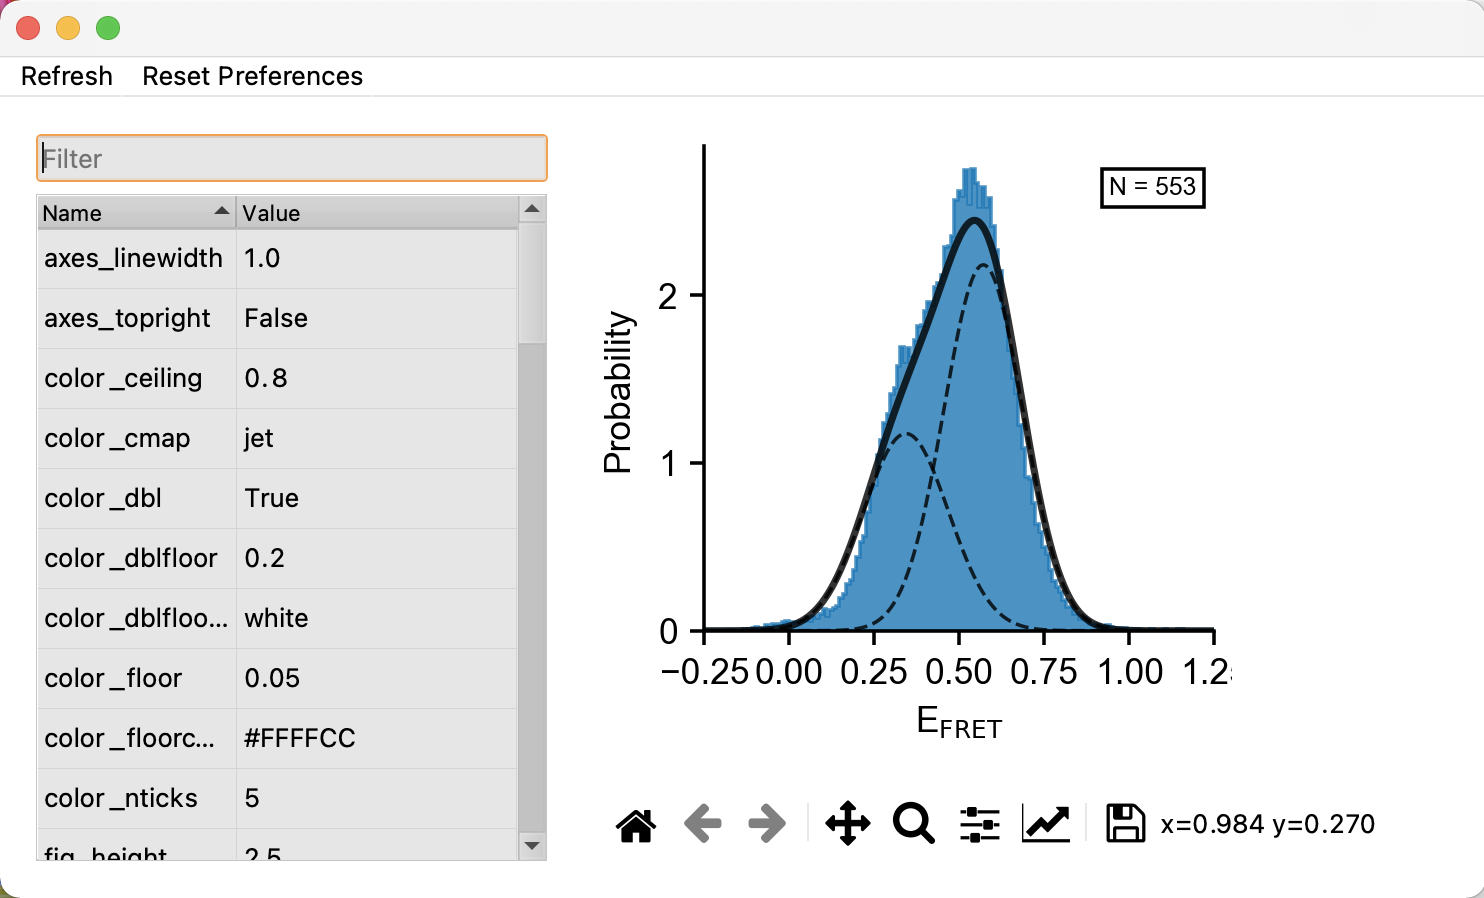
\includegraphics[scale=0.38]{1D Histofigure.png}
     \caption{A typical one dimensional histogram. Note the number of traces used N in the top right. If a model has been calculated, a population-weighted set of emission distributions is plotted as the solid black with the dotted lines as the individual populations. These lines are not a Gaussian fit of the data, but come directly from the models. Theoretically, better models/processing will result in a better fit of the histogram.}
     \label{fig:my_label}
 \end{figure}

 Notable preferences the user might want to change include:
\begin{itemize}
    \item Hist$\_$Force$\_$y to force the y axis value
    \item Hist$\_$log$\_$y puts the y-axis in log scale
    \item model$\_$on will toggle the model as described in figure 9
    \item hist$\_$false toggles the histogram itself, blue in the figure
    \item hist$\_$color will change the color of the histogram
\end{itemize}
The save icon below the graph can be used to export the figure. 

\section{Two-Dimensional Histograms}
The two-dimensional histograms in tMAVEN also have the axis of time. Generate by navigating Plots/\textbf{FRET hist 2D} The histogram is automatically smoothed by a median  filter which setting can be changed (see below). One of the most useful capabilities is the choice of using post-synchronization. In this case, t=0 represents the time of transition from one specified state to another, see below. Note that post-synch can only operate once a model is run and transitions have been detected. \\ \\ \\ \\
\begin{figure} [t]
    \centering
    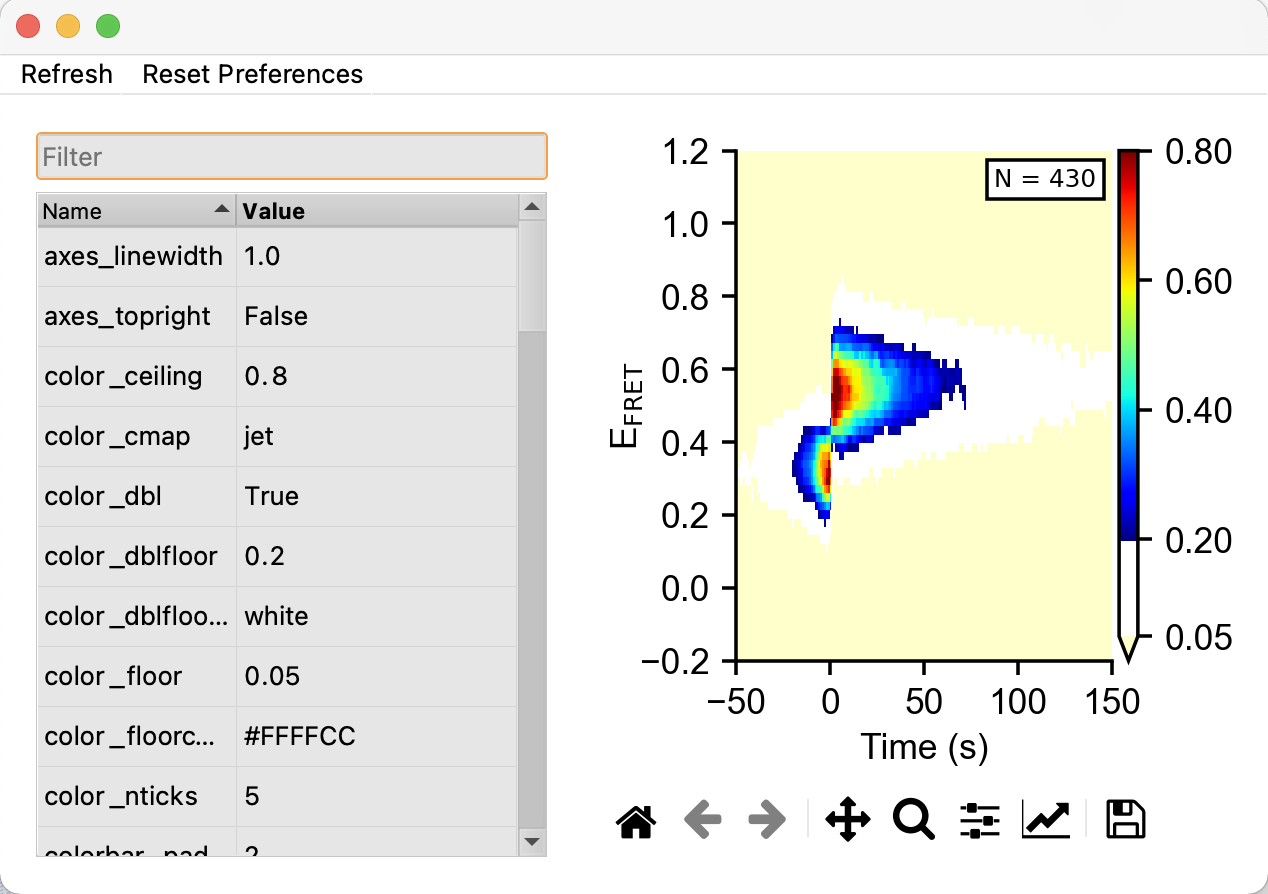
\includegraphics[scale=0.38]{2dHistoPostSyncFigure.png}
    \caption{A two dimensional histogram with post-sync on using the het color map.}
    \label{fig:my_label}

\end{figure}

\vspace*{-40pt}

Useful preferences:

\begin{itemize}
    \item $\_$ceiling sets the ceiling for the color mapping
    \item Color$\_$dbl enables two floors
    \item Color$\_$floor$\_$color is the lower floor 
    \item $\_$cmap determines the color map, all matplotlib maps are supported
    \item hist$\_$smooth$\_$med toggles the use of a median filter on the graph and hist$\_$smoothx/y determine the widths of this filter
    \item time$\_$dt changes the time ticks, set to acquisition time to yield the same axis as traces while time$\_$nbins changes the length of time shown. 
    \item hist$\_$normalizeframe will normalize the histogram to mitigate photobleaching or additional transition at different times, see figure 11.
\end{itemize}
For post synchronization, tMAVEN will use the existing model which has identified transitions so users can essentially monitor all traces after a specific transition in a data set. Notice that N, number of traces used, will likely change since not all traces have all transitions. Small n represents the number of transitions measured not number of traces.   
\begin{itemize}
    \item sync$\_$postsync toggles post synchronization
    \item sync$\_$singledwell set to true shows only the dwell before and after transition. In other words, a false setting will also show future transitions. 
    \item sync$\_$hmmstate$\_$1 shows the pretransition state while sync$\_$hmmstate$\_$2 shows the post transition state, input "-1" for any other state
\end{itemize}

\begin{figure} [h]
    \centering
    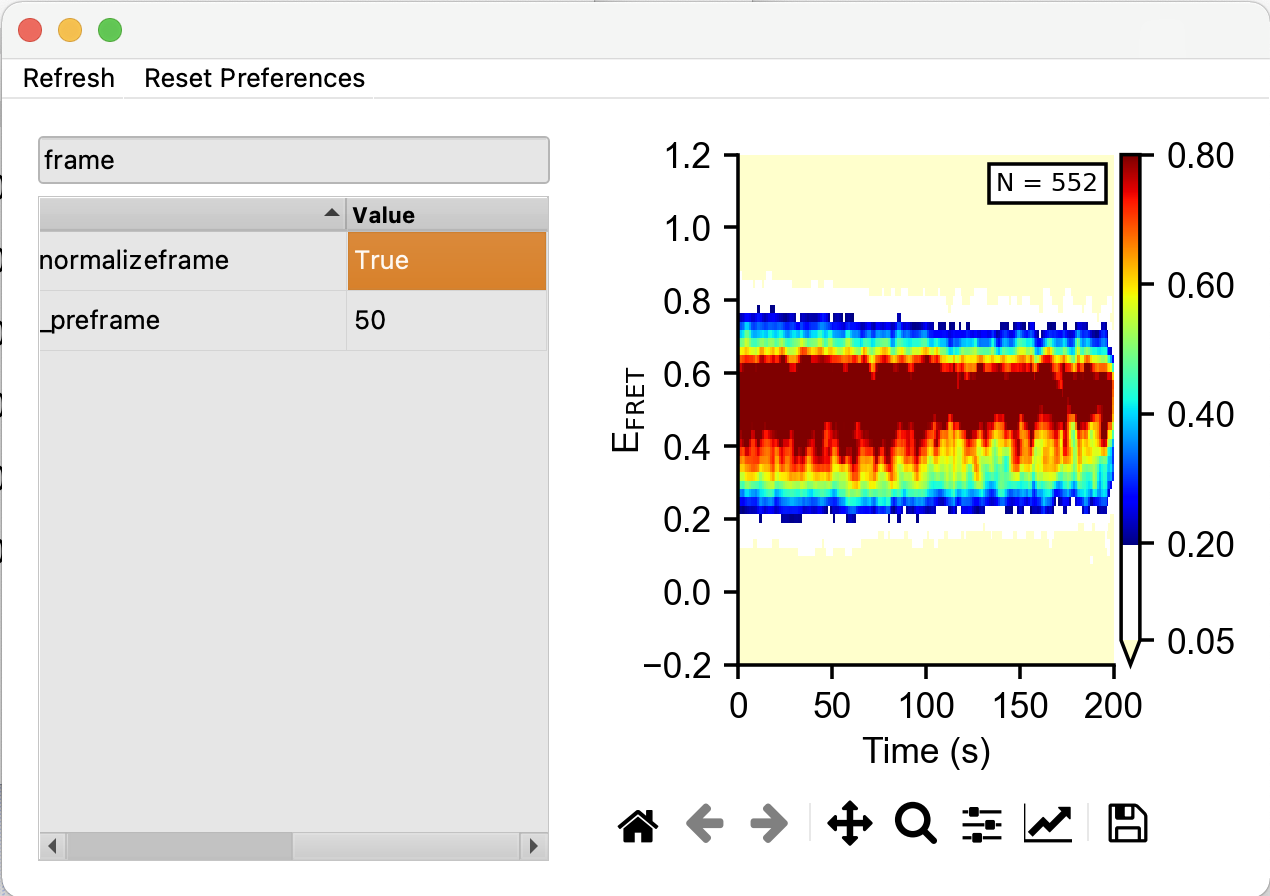
\includegraphics[scale=0.34]{NormalizedFigure.png}
    \caption{The same graph as figure 10 with normalization on.}
    \label{fig:my_label}
\end{figure}


\printbibliography

\end{document}